\documentclass{paper}
\usepackage{hyperref}
\usepackage{floatrow}
\usepackage{graphicx}
\usepackage[
backend=biber,
style=numeric,
sorting=nty
]{biblatex}

\graphicspath{{./images/}}
\addbibresource{refs.bib}

\title{TBD}
\author{Viktor Horsmanheimo}
\date{\today}

\begin{document}
\maketitle
\tableofcontents
\newpage

\begin{abstract}
    In this paper we're going to give an overview about FPGAs and cryptographic
    schemes
\end{abstract}

\section{Introduction}
Field programmable gate arrays(FPGA) have become more popular in the past few
decades. FPGAs are chips that unlike standard ones for example
CPUs, are programmable after manufacturing. FPGAs consist of logic gate arrays
which evaluate simple boolean function. Between these gates we have wires
and control blocks which allows the data to be moved between the logic gates.
We will present the internals of these components in the next section.

FPGAs were created in the 80s by Altera, at that time they weren't very
practical because the size of the transistors were very large. This meant that
you couldn't fit very much on a reasonably sized chip. Moore's law states that
the transistor size halves every two years, this has affected FPGAs as well and
now they contain enough transistors to compete with application specific
integrated circuits (ASIC). ASICs are hardware that is made specifically for a
task, for example cryptographic currency mining hardware. These chips are in
general faster than FPGAs if you are working with the latest technology. Due to
the fact that it is risky to work with the newest technology, manufacturers
rarely use it. This is where FPGAs are useful, since they're reprogrammable
they can always use the latest technology. If something goes wrong you can
always change it. Because of this FPGAs continue to rise in popularity. % TODO add picture of ASIC vs FPGA nano meters

% TODO add introduction to actual topic when intro is done

\section{Outline}
In section \ref{FPGA_introduction} we will go into detail about how FPGAs work
internally, how they're configured and the technologies behind it.

\section{FPGA}
\label{FPGA_introduction}

As briefly mentioned in the introduction, FPGAs consisting of logic gates. In
this section we will give an overview about how they and other the other
components work and what different ways there are to configure these chips.

Modern FPGAs may also include a number of other components, for example
processors and multipliers though we will not cover those.

\subsection{Components}
\subsubsection{Lookup tables}

In boolean algebra we can represent a function as a truth table of size $2^N$.
This translates directly to binary and because of this property FPGAs
extensively use lookup tables(LUT). The way LUTs are implemented are using
$N:1$ multiplexers and $N$-bits of memory, you store all the answers of the LUT
in memory. Then the multiplexer takes $N$ inputs and maps it to the LUTs
answer. For example if we have the following function.

$$A + B \times C$$

There are $2^3 = 8$ different answers to the function. We then
store all of these answers in memory in a table as similar to what is seen in
table \ref{tab:example_truth_table}.

\begin{table}[ht]
    \centering
    \begin{tabular}{|l|l|l|l|}
        \hline
        A & B & C & Out \\ \hline
        0 & 0 & 0 & 0   \\ \hline
        0 & 0 & 1 & 1   \\ \hline
        0 & 1 & 0 & 0   \\ \hline
        0 & 1 & 1 & 1   \\ \hline
        1 & 0 & 0 & 0   \\ \hline
        1 & 0 & 1 & 1   \\ \hline
        1 & 1 & 0 & 1   \\ \hline
        1 & 1 & 1 & 1   \\ \hline
    \end{tabular}
    \caption{Example truth table}
    \label{tab:example_truth_table}
\end{table}

% flip flops
This alone isn't enough to be able to implement everything as we cannot store
state. What we need is some way to store information, this is where delay(D)
flip-flops come in. Here we have an example of how an FPGA might use a
flip-flop \ref{Fig:lut_flipflop}. They can store a single bit of data, with
this the chip can store state and is now complete.

\begin{figure}[H]
    \centering
    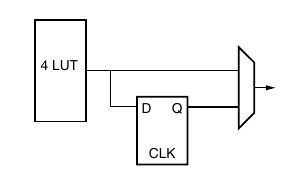
\includegraphics[scale=0.6]{lookup_table_flipflop.png}
    \caption{An example of how a lookup table could be implemented\cite{m_d_mano_digital_2012}}
    \label{Fig:lut_flipflop}
\end{figure}

These LUTs are what allow for FPGAs to be reconfigured. By simply writing to
the tables the correct values it allows the chip to implement any function.
There's been studies done about how many LUTs a logic block should contain, if
there were more LUTs it would allow for more complex logic. Though adding more
inputs would also make the chip slower\cite{amano_principles_2018}.

\begin{figure}[H]
    \label{fig:fpga_structure}
    \caption{An example of an island-style FPGA\cite{m_d_mano_digital_2012}}
    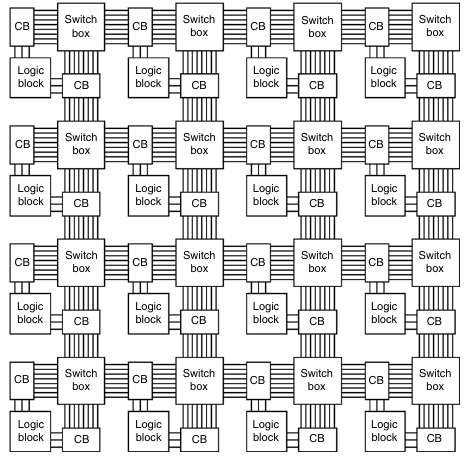
\includegraphics[scale=0.7]{fpga_structure.png}
\end{figure}

\subsubsection{Input/Output blocks}
Input/Output blocks (I/O blocks, IOB) are blocks that are placed around the
periphery of the FPGA. They control the interface between the FPGA and external
circuits such as the clock and power usage.

\subsubsection{Connection block}
Along the wires by the logic blocks there are connection blocks (CB). These blocks
control which data goes into and out of a logic block. They also connect the
I/O blocks to the FPGA.

\subsubsection{Switch block}
A switch block (switch box, SB) is a type of block that exists at every intersection in the wiring.
As the name suggests it's built from a bunch of switches and it's job is to
route the electricity between the logic blocks. There are different types of
switch blocks, depending on the type it will have different levels of
connectivity and efficiency. Though the specifics of this is out of the scope
of this paper.


\subsection{Configuration}
There are various ways reprogrammability can be implemented, though we're only
going to focus on the three main technologies: static RAM, flash memory and
antifuse.

\subsubsection{Static RAM}
Static RAM (SRAM) is a very simple one, you store the configuration in SRAM.

\subsubsection{Flash memory}
\subsubsection{Antifuse}

\printbibliography

\end{document}
